\documentclass[11pt,a4paper]{article}
\usepackage[margin=1in]{geometry}
\usepackage[T1]{fontenc}
\usepackage[utf8]{inputenc}
\usepackage{lmodern}
\usepackage{microtype}
\usepackage{xcolor}
\usepackage{booktabs,array,longtable,tabularx}
\usepackage{enumitem}
\usepackage{amsmath,amssymb}
\usepackage{fancyhdr}
\usepackage{hyperref}
\usepackage{titlesec}
\usepackage{listings}
\usepackage{inconsolata}
\usepackage{needspace}
\usepackage{tikz}
\usetikzlibrary{arrows.meta,positioning,fit,shapes.multipart}
\hypersetup{colorlinks=true,linkcolor=blue!50!black,urlcolor=blue!50!black}
\definecolor{accent}{RGB}{33,91,163}
\definecolor{soft}{RGB}{242,246,252}
\definecolor{softline}{RGB}{214,224,238}
\definecolor{codebg}{RGB}{248,248,248}
\pagestyle{fancy}
\fancyhf{}
\lhead{microMC nuclear data guide}
\rhead{\thepage}
\setlength{\headheight}{14pt}
\titleformat{\section}{\Large\bfseries\color{accent}}{\thesection}{0.6em}{}
\titleformat{\subsection}{\large\bfseries\color{accent}}{\thesubsection}{0.6em}{}
\titleformat{\subsubsection}{\normalsize\bfseries\color{accent}}{\thesubsubsection}{0.6em}{}
\lstset{basicstyle=\ttfamily\small,backgroundcolor=\color{codebg},frame=single,framerule=0pt,breaklines=true,columns=fullflexible}

\begin{document}

\begin{titlepage}
\centering
\vspace*{2.0cm}
{\Huge\bfseries microMC Nuclear Data Structures\\[0.35em]}
{\Large A rigorous guide using a small but faithful toy library\\}
\vspace{1.3cm}
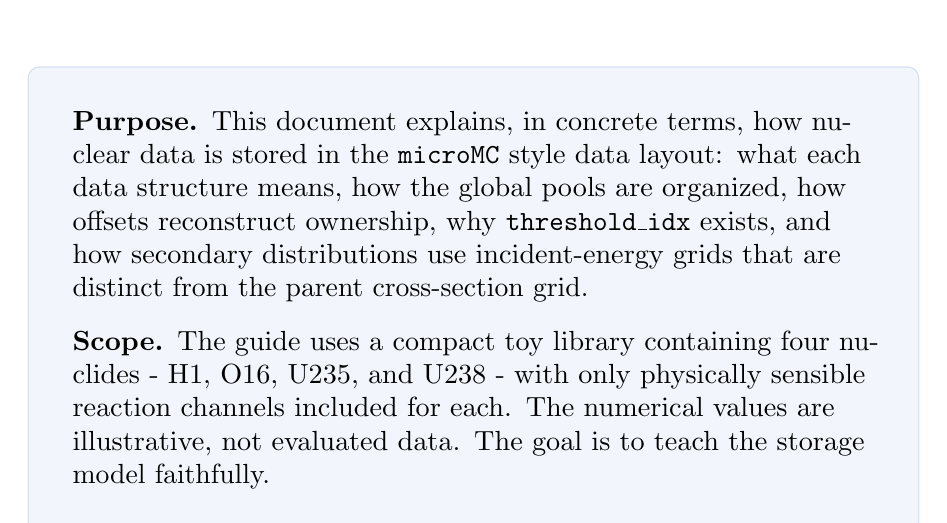
\begin{tikzpicture}
\node[draw=softline, fill=soft, rounded corners=4pt, inner sep=16pt, text width=0.84\textwidth] {
\textbf{Purpose.} This document explains, in concrete terms, how nuclear data is stored in the \texttt{microMC} style data layout: what each data structure means, how the global pools are organized, how offsets reconstruct ownership, why \texttt{threshold\_idx} exists, and how secondary distributions use incident-energy grids that are distinct from the parent cross-section grid.\\[0.75em]
\textbf{Scope.} The guide uses a compact toy library containing four nuclides - H1, O16, U235, and U238 - with only physically sensible reaction channels included for each. The numerical values are illustrative, not evaluated data. The goal is to teach the storage model faithfully.
};
\end{tikzpicture}
\vfill
{\large Compiled from LaTeX for reference and annotation}
\vspace*{1.4cm}
\end{titlepage}

\tableofcontents
\newpage

\section{How to read this document}
This guide is intentionally concrete. It does not start from abstract software architecture. It starts from the actual questions that matter when reading or writing the code:
\begin{itemize}[leftmargin=1.4em]
  \item What is owned directly, and what is only referenced indirectly?
  \item What does each field in each structure actually mean?
  \item Why are there offsets everywhere?
  \item What is the difference between a parent nuclide energy grid and a secondary-distribution incident-energy grid?
  \item When a neutron interacts with a nuclide, how do the structures get traversed in practice?
  \item How does the code sample a reaction and process the collision?
\end{itemize}
The toy library is small enough to inspect by eye, but it keeps the important structural features:
\begin{itemize}[leftmargin=1.4em]
  \item each nuclide has its own parent cross-section grid,
  \item reactions only use slices of that parent grid,
  \item secondary distributions have independent incident-energy grids,
  \item fission needs more than one auxiliary pool (prompt spectrum, $\bar\nu$, delayed groups),
  \item aggregate channels such as non-fission absorption require care.
\end{itemize}

\section{The central idea of the storage model}
The design avoids nested ownership. In a naive object model you might expect the following:
\begin{lstlisting}
Nuclide
  owns energy grid
  owns reactions
    each reaction owns xs array
    each reaction owns angular law
    each reaction owns outgoing-energy law
\end{lstlisting}
That is \emph{not} how this layout works. Instead, the design uses:
\begin{enumerate}[leftmargin=1.4em]
  \item a few large global arrays (energy grids, cross sections, secondary tables), and
  \item small descriptor structures that say where each relevant slice begins and how long it is.
\end{enumerate}
So a reaction does not ``contain'' its cross section table. A reaction descriptor says, in effect, ``my cross section values begin at offset 148 in the global \texttt{xs\_pool}, my table has length 12, and the first value corresponds to parent-grid index 4.''

\subsection{Why this is useful}
This gives several practical benefits:
\begin{itemize}[leftmargin=1.4em]
  \item compact storage,
  \item no deep heap allocation tree,
  \item easy serialization to a binary file,
  \item easier transfer to accelerators (the \texttt{NuclearData} view struct is pure POD),
  \item one consistent lookup strategy based on offsets.
\end{itemize}
The price is that the code can look alien at first. It is much more like an indexing system than like classical object-oriented encapsulation.

\subsection{The two struct tiers: owner and view}
\texttt{NuclearDataHost} owns the heap via \texttt{std::vector} members. It is never passed to physics routines. Instead, \texttt{host.view()} returns a \texttt{NuclearData} struct whose fields are raw pointers into those vectors. \texttt{NuclearData} is pure POD --- no \texttt{std::} types --- so it can be \texttt{memcpy}'d to GPU device memory unchanged. All physics code takes \texttt{const NuclearData\&}.

\section{The three different kinds of energy grid}
A major source of confusion is the word ``energy grid.'' There is not just one of them.

\subsection{Parent nuclide cross-section grid}
Each nuclide has its own parent cross-section grid. This is the grid stored in the global \texttt{energy\_grids} pool and referenced by a \texttt{NuclideDescriptor}. Reaction cross sections are aligned against this parent grid using \texttt{threshold\_idx}.

\subsection{Reaction support on the parent grid}
A reaction usually does not use the whole parent grid. Instead it uses a suffix or other contiguous slice of it. This support is not stored as a separate energy array. It is implied by three things:
\begin{itemize}[leftmargin=1.4em]
  \item the parent grid,
  \item \texttt{threshold\_idx},
  \item \texttt{xs\_length}.
\end{itemize}
If the parent grid has 9 points and a reaction has \texttt{threshold\_idx = 4}, \texttt{xs\_length = 5}, then the reaction occupies parent local indices 4 through 8.

\subsection{Secondary-distribution incident-energy grids}
Angular laws, continuum/Kalbach distributions, fission outgoing-energy distributions, and $\bar\nu(E)$ laws all have their own incident-energy grids. These should not be assumed equal to the parent grid. In practice they are often much coarser and placed only where the secondary law changes enough to justify tabulation.

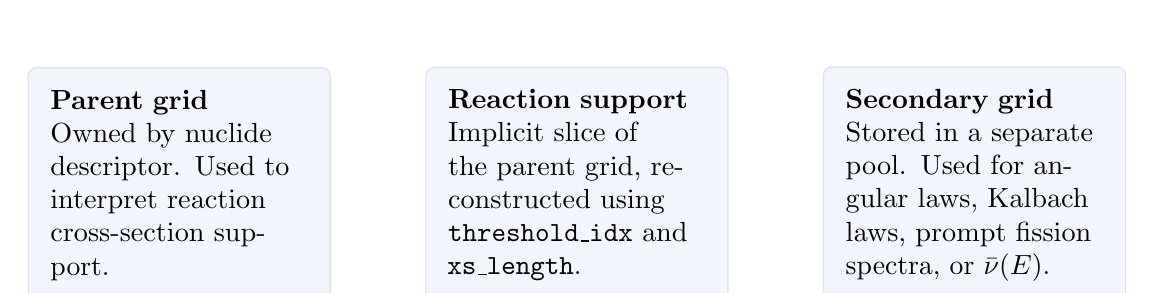
\begin{tikzpicture}[node distance=8mm and 12mm]
\node[draw=softline, fill=soft, rounded corners=3pt, inner sep=8pt, text width=0.27\textwidth] (a) {\textbf{Parent grid}\\Owned by nuclide descriptor. Used to interpret reaction cross-section support.};
\node[draw=softline, fill=soft, rounded corners=3pt, inner sep=8pt, text width=0.27\textwidth, right=of a] (b) {\textbf{Reaction support}\\Implicit slice of the parent grid, reconstructed using \texttt{threshold\_idx} and \texttt{xs\_length}.};
\node[draw=softline, fill=soft, rounded corners=3pt, inner sep=8pt, text width=0.27\textwidth, right=of b] (c) {\textbf{Secondary grid}\\Stored in a separate pool. Used for angular laws, Kalbach laws, prompt fission spectra, or $\bar\nu(E)$.};
\end{tikzpicture}

\section{The toy library used throughout}
The toy library contains four nuclides with intentionally different parent grids.

\subsection{Parent grids}
\begin{longtable}{>{\ttfamily}p{1.7cm} p{10.5cm}}
\toprule
Nuclide & Parent cross-section grid \\
\midrule
H1 & [1e-5, 1e-3, 1e-1, 1e0, 1e2, 1e4, 1e6] \\
O16 & [1e-3, 1e-1, 1e0, 1e1, 1e3, 1e5, 1e6, 1e7] \\
U235 & [1e-5, 1e-3, 1e-1, 1e0, 1e1, 1e3, 1e4, 1e5, 1e6] \\
U238 & [1e-5, 1e-2, 1e0, 1e2, 1e3, 1e5, 1e6, 1e7, 2e7] \\
\bottomrule
\end{longtable}

The global \texttt{energy\_grids} pool is just the concatenation of these four arrays.

\begin{lstlisting}
energy_grids = [
  // H1: indices 0..6
  1e-5, 1e-3, 1e-1, 1e0, 1e2, 1e4, 1e6,
  // O16: indices 7..14
  1e-3, 1e-1, 1e0, 1e1, 1e3, 1e5, 1e6, 1e7,
  // U235: indices 15..23
  1e-5, 1e-3, 1e-1, 1e0, 1e1, 1e3, 1e4, 1e5, 1e6,
  // U238: indices 24..32
  1e-5, 1e-2, 1e0, 1e2, 1e3, 1e5, 1e6, 1e7, 2e7
]
\end{lstlisting}

\subsection{Reaction inventory}
Only channels that are physically meaningful for each nuclide are included. Note that in the actual \texttt{microMC} codebase, non-fission absorption (MT=102--117) is stored as a single summed \texttt{ABSORPTION} channel. There is no separate ``capture'' reaction --- capture is folded into absorption. The toy library follows this convention:
\begin{longtable}{>{\ttfamily}p{1.7cm} p{10.8cm}}
\toprule
Nuclide & Included reactions \\
\midrule
H1 & elastic, absorption \\
O16 & elastic, discrete inelastic, continuum inelastic, absorption, n2n, n3n \\
U235 & elastic, discrete inelastic, continuum inelastic, fission, absorption, n2n, n3n \\
U238 & elastic, discrete inelastic, continuum inelastic, fission, absorption, n2n, n3n \\
\bottomrule
\end{longtable}

\section{Direct explanation of each core data structure}
This section explains each structure directly, field by field, in plain language.

\subsection{\texttt{NuclideDescriptor}}
This structure answers two questions:
\begin{itemize}[leftmargin=1.4em]
  \item where does this nuclide's parent cross-section grid live?
  \item where does this nuclide's reaction block live?
\end{itemize}

\begin{longtable}{p{2.3cm} p{10.0cm}}
\toprule
Field & Meaning \\
\midrule
\texttt{grid\_offset} & Starting index of this nuclide's parent energy grid inside the global \texttt{energy\_grids} pool. \\
\texttt{grid\_length} & Number of energy points in the parent grid. \\
\texttt{A} & Atomic mass ratio (target mass / neutron mass). Used for kinematics. \\
\texttt{rxn\_offset} & Starting index of this nuclide's reaction block in the global \texttt{reactions} array. \\
\texttt{n\_reactions} & Number of reactions owned by this nuclide. \\
\texttt{zaid} & ZAID identifier (e.g.\ 1001 for H1, 92238 for U238). \\
\bottomrule
\end{longtable}

For the toy library:
\begin{lstlisting}
nuclides[0] = { grid_offset=0,  grid_length=7, A=1.0,   rxn_offset=0,  n_reactions=2, zaid=1001  }
nuclides[1] = { grid_offset=7,  grid_length=8, A=16.0,  rxn_offset=2,  n_reactions=6, zaid=8016  }
nuclides[2] = { grid_offset=15, grid_length=9, A=235.0, rxn_offset=8,  n_reactions=7, zaid=92235 }
nuclides[3] = { grid_offset=24, grid_length=9, A=238.0, rxn_offset=15, n_reactions=7, zaid=92238 }
\end{lstlisting}
This means, for example, that U235 owns:
\begin{itemize}[leftmargin=1.4em]
  \item \texttt{energy\_grids[15..23]}, and
  \item \texttt{reactions[8..14]}.
\end{itemize}

\subsection{\texttt{ReactionDescriptor}}
This structure answers three questions:
\begin{itemize}[leftmargin=1.4em]
  \item where do this reaction's cross-section values live?
  \item where do they begin on the parent grid?
  \item where is the reaction's outgoing-data metadata stored?
\end{itemize}

\begin{longtable}{p{2.4cm} p{9.9cm}}
\toprule
Field & Meaning \\
\midrule
\texttt{type} & Reaction category. One of: \texttt{ELASTIC}, \texttt{DISCRETE\_INELASTIC}, \texttt{CONTINUUM\_INELASTIC}, \texttt{FISSION}, \texttt{ABSORPTION}, \texttt{N2N}, \texttt{N3N}. \\
\texttt{xs\_offset} & Starting index in the global \texttt{xs\_pool} where this reaction's tabulated cross-section values begin. \\
\texttt{xs\_length} & Number of tabulated cross-section values for this reaction. \\
\texttt{threshold\_idx} & Parent-grid local index corresponding to the first cross-section entry. This is the key field that reconstructs reaction support on the parent grid. \\
\texttt{dist\_id} & Index into the relevant outgoing-distribution pool. Which pool depends on reaction type (see below). Set to $-1$ for absorption (no secondaries). \\
\texttt{Q\_value} & Reaction Q-value in eV. Only physically meaningful for discrete inelastic. \\
\texttt{multiplicity} & Number of outgoing neutrons. 1 for elastic/inelastic, 2 for (n,2n), 3 for (n,3n), $-1$ for fission (energy-dependent $\bar\nu$). \\
\texttt{yield\_id} & Index into the \texttt{FissionYieldPool}. Only meaningful for fission ($-1$ otherwise). \\
\texttt{delayed\_id} & Index into \texttt{delayed\_fission\_descs}. Only meaningful for fission ($-1$ otherwise). \\
\bottomrule
\end{longtable}

\subsubsection{What \texttt{dist\_id} points to, by reaction type}
The \texttt{dist\_id} field is polymorphic. Its target pool depends on the reaction type:

\begin{longtable}{p{4.0cm} p{4.5cm} p{3.5cm}}
\toprule
Reaction type & Pool indexed by \texttt{dist\_id} & What is sampled \\
\midrule
\texttt{ELASTIC} & \texttt{data.angular} & scattering cosine $\mu_\text{cm}$ \\
\texttt{DISCRETE\_INELASTIC} & \texttt{data.angular} & scattering cosine $\mu_\text{cm}$ \\
\texttt{CONTINUUM\_INELASTIC} & \texttt{data.kalbach} & $E'_\text{out}$ and $\mu$ \\
\texttt{FISSION} & \texttt{data.fission\_energy} & outgoing energy $E'$ \\
\texttt{N2N}, \texttt{N3N} & \texttt{data.kalbach} & $E'_\text{out}$ and $\mu$ \\
\texttt{ABSORPTION} & --- (unused) & nothing ($\texttt{dist\_id} = -1$) \\
\bottomrule
\end{longtable}

The \texttt{switch} in the transport loop dispatches to the correct collision handler, which knows which pool to pass \texttt{dist\_id} into. For example, \texttt{elastic\_scatter} calls \texttt{sample\_cosine(data.angular, rxn.dist\_id, ...)}, while \texttt{inelastic\_scatter\_cont} calls \texttt{sample\_kalbach\_mann(data.kalbach, rxn.dist\_id, ...)}.

\subsection{\texttt{AngularDistPool} --- the two-level ragged array}
\label{sec:angular-pool}
This pool stores angular laws for elastic and discrete inelastic reactions. Logically, one angular distribution looks like this:
\begin{lstlisting}
Distribution k:
  incident energy E1 -> mu/pdf/cdf table T1  (n1 bins)
  incident energy E2 -> mu/pdf/cdf table T2  (n2 bins)
  incident energy E3 -> mu/pdf/cdf table T3  (n3 bins)
\end{lstlisting}

The pool flattens this ragged structure into global arrays using two levels of indirection:
\begin{itemize}[leftmargin=1.4em]
  \item \textbf{Level 1:} \texttt{energy\_offsets[k]} to \texttt{energy\_offsets[k+1]} gives the range of incident-energy entries belonging to distribution \texttt{k}. The actual energy values are in the \texttt{energies} array at those positions.
  \item \textbf{Level 2:} For each incident-energy entry \texttt{j}, \texttt{table\_offsets[j]} to \texttt{table\_offsets[j+1]} gives the range of $\mu$/pdf/cdf bins belonging to that entry.
\end{itemize}

\subsubsection{Concrete example with offsets}
Suppose distribution 0 (H1 elastic) has 3 incident energies, each with a different number of $\mu$ bins, and distribution 1 (O16 elastic) has 2 incident energies:

\begin{lstlisting}
Dist 0 (H1 elastic):
  E=1e-3 -> 5 mu bins
  E=1e2  -> 5 mu bins
  E=1e6  -> 8 mu bins

Dist 1 (O16 elastic):
  E=1e-1 -> 5 mu bins
  E=1e5  -> 6 mu bins
\end{lstlisting}

The flattened arrays would be:

\begin{lstlisting}
energy_offsets = [0, 3, 5, ...]
                  |  |  |
                  |  |  +-- dist 2 starts at energy entry 5
                  |  +-- dist 1 starts at energy entry 3
                  +-- dist 0 starts at energy entry 0

energies = [1e-3, 1e2, 1e6,   1e-1, 1e5,   ...]
            |---- dist 0 ---|  |- dist 1 -|

table_offsets = [0, 5, 10, 18,   23, 29, ...]
                 |  |   |   |     |   |
                 |  |   |   |     |   +-- end of dist1/E=1e5 (6 bins)
                 |  |   |   |     +-- start of dist1/E=1e5
                 |  |   |   +-- end of dist0/E=1e6 (8 bins)
                 |  |   +-- start of dist0/E=1e6
                 |  +-- start of dist0/E=1e2 (5 bins)
                 +-- start of dist0/E=1e-3 (5 bins)

mu  = [mu values for all tables, concatenated]
pdf = [pdf values for all tables, concatenated]
cdf = [cdf values for all tables, concatenated]
\end{lstlisting}

To sample from distribution $k$ at incident energy $E$:
\begin{enumerate}[leftmargin=1.4em]
  \item Use \texttt{energy\_offsets[k]} and \texttt{energy\_offsets[k+1]} to find the range of incident energies.
  \item Use stochastic energy interpolation (section~\ref{sec:stoch-interp}) to pick one incident-energy entry $j$.
  \item Use \texttt{table\_offsets[j]} and \texttt{table\_offsets[j+1]} to find the $\mu$/cdf slice.
  \item Sample from the CDF to get the scattering cosine.
\end{enumerate}

\subsection{\texttt{EnergyDistPool}}
This pool stores outgoing-energy laws tabulated at incident energies. It is used for prompt fission spectra and delayed fission spectra. The structure is identical to the angular pool:
\begin{itemize}[leftmargin=1.4em]
  \item \texttt{energy\_offsets} $\to$ \texttt{energies}: which incident energies belong to each distribution,
  \item \texttt{table\_offsets} $\to$ \texttt{E\_out}/\texttt{pdf}/\texttt{cdf}: the outgoing-energy tables for each incident energy.
\end{itemize}
The same two-level ragged array pattern, the same access logic. Only the leaf data differs ($E'_\text{out}$ instead of $\mu$).

\subsection{\texttt{KalbachMannDistPool}}
This pool is a specialised version of an outgoing-energy distribution pool. It has the same two-level structure as \texttt{EnergyDistPool}, but the leaf tables store two extra arrays: the Kalbach-Mann parameters \texttt{r} and \texttt{a}. These are stored parallel to \texttt{E\_out}/\texttt{pdf}/\texttt{cdf}, indexed by the same \texttt{table\_offsets}. Channels like continuum inelastic, (n,2n), and (n,3n) use this pool.

\subsection{\texttt{FissionYieldDescriptor} and \texttt{FissionYieldPool}}
This pool stores tabulated $\bar\nu(E)$ laws. One entry is logically just a pair of arrays:
\begin{lstlisting}
energy  = [E1, E2, E3, ...]
nu_bar  = [v1, v2, v3, ...]
\end{lstlisting}
The descriptor tells you where a particular law begins in the global \texttt{fy\_energy} and \texttt{fy\_nu\_bar} arrays and how many points it has. This is a single-level indirection --- simpler than the angular/energy pools because $\bar\nu$ is a scalar function of $E$, not a distribution.

\subsection{\texttt{DelayedNeutronGroupDescriptor} and \texttt{DelayedFissionDescriptor}}
These structures let a fission reaction reference delayed neutron metadata compactly. The chain is:
\begin{enumerate}[leftmargin=1.4em]
  \item The reaction's \texttt{delayed\_id} points to a \texttt{DelayedFissionDescriptor}.
  \item The \texttt{DelayedFissionDescriptor} has \texttt{group\_offset} and \texttt{n\_groups}, giving a slice of the \texttt{delayed\_groups} array.
  \item Each \texttt{DelayedNeutronGroupDescriptor} in that slice has:
  \begin{itemize}
    \item \texttt{yield\_id} --- index into \texttt{FissionYieldPool} for this group's $\bar\nu_d(E)$,
    \item \texttt{dist\_id} --- index into \texttt{data.delayed\_fission\_energy} (an \texttt{EnergyDistPool}) for this group's delayed spectrum.
  \end{itemize}
\end{enumerate}

\subsection{\texttt{Material}}
\label{sec:material}
A material binds nuclides together with number densities and a temperature. It is not part of the nuclear data --- it is a user-defined composition.

\begin{longtable}{p{3.5cm} p{8.8cm}}
\toprule
Field & Meaning \\
\midrule
\texttt{name} & Human-readable label. \\
\texttt{density} & Input density. Negative = mass density (g/cm$^3$), positive = atomic density (atoms/barn-cm), zero = direct number densities. \\
\texttt{temperature} & Material temperature in Kelvin. Used for target motion sampling. \\
\texttt{zaids[]} & Array of ZAID identifiers for each nuclide in the mix. \\
\texttt{number\_quantity[]} & Input atom or mass fractions (sign determines interpretation). \\
\texttt{n\_nuclides} & Number of active nuclides. \\
\texttt{number\_densities[]} & Computed by \texttt{resolve\_material}: absolute number densities $N_i$ in atoms/barn-cm. \\
\texttt{nuclide\_ids[]} & Computed by \texttt{resolve\_material}: index into \texttt{NuclearData::nuclides[]} for each ZAID. \\
\bottomrule
\end{longtable}

\texttt{resolve\_material(mat, data)} does two things: (1) maps each ZAID to its index in the nuclear data, and (2) converts the input density and fractions into absolute number densities using atomic masses from the ENDF/B-VII.1 table. All subsequent physics uses \texttt{number\_densities[]} and \texttt{nuclide\_ids[]}.

\section{The toy reaction supports}
This section records where each reaction begins on its parent grid. This is what \texttt{threshold\_idx} and \texttt{xs\_length} encode.

\subsection{H1}
Parent grid length: 7
\begin{longtable}{p{3.3cm} p{2cm} p{2cm} p{4.3cm}}
\toprule
Reaction & thr idx & xs len & Parent local support \\
\midrule
elastic & 0 & 7 & 0..6 \\
absorption & 2 & 5 & 2..6 \\
\bottomrule
\end{longtable}

\subsection{O16}
Parent grid length: 8
\begin{longtable}{p{3.3cm} p{2cm} p{2cm} p{4.3cm}}
\toprule
Reaction & thr idx & xs len & Parent local support \\
\midrule
elastic & 0 & 8 & 0..7 \\
discrete inelastic & 3 & 5 & 3..7 \\
continuum inelastic & 4 & 4 & 4..7 \\
absorption & 2 & 6 & 2..7 \\
n2n & 4 & 4 & 4..7 \\
n3n & 5 & 3 & 5..7 \\
\bottomrule
\end{longtable}

\subsection{U235}
Parent grid length: 9
\begin{longtable}{p{3.3cm} p{2cm} p{2cm} p{4.3cm}}
\toprule
Reaction & thr idx & xs len & Parent local support \\
\midrule
elastic & 0 & 9 & 0..8 \\
discrete inelastic & 3 & 6 & 3..8 \\
continuum inelastic & 4 & 5 & 4..8 \\
fission & 2 & 7 & 2..8 \\
absorption & 2 & 7 & 2..8 \\
n2n & 4 & 5 & 4..8 \\
n3n & 5 & 4 & 5..8 \\
\bottomrule
\end{longtable}

\subsection{U238}
Parent grid length: 9
\begin{longtable}{p{3.3cm} p{2cm} p{2cm} p{4.3cm}}
\toprule
Reaction & thr idx & xs len & Parent local support \\
\midrule
elastic & 0 & 9 & 0..8 \\
discrete inelastic & 3 & 6 & 3..8 \\
continuum inelastic & 4 & 5 & 4..8 \\
fission & 3 & 6 & 3..8 \\
absorption & 2 & 7 & 2..8 \\
n2n & 4 & 5 & 4..8 \\
n3n & 5 & 4 & 5..8 \\
\bottomrule
\end{longtable}

\section{The global \texttt{reactions[]} array in the toy library}
The reactions are laid out nuclide by nuclide.

\begin{longtable}{>{\ttfamily}p{1.1cm} p{3.0cm} p{1.8cm} p{1.6cm} p{1.8cm} p{3.2cm}}
\toprule
Idx & Reaction & xs offset & xs len & thr idx & Notes \\
\midrule
0 & H1 elastic & 0 & 7 & 0 & angular dist 0 \\
1 & H1 absorption & 7 & 5 & 2 & dist\_id = $-1$ \\
2 & O16 elastic & 12 & 8 & 0 & angular dist 1 \\
3 & O16 disc inel & 20 & 5 & 3 & angular dist 2 \\
4 & O16 cont inel & 25 & 4 & 4 & Kalbach dist 0 \\
5 & O16 absorption & 29 & 6 & 2 & dist\_id = $-1$ \\
6 & O16 n2n & 35 & 4 & 4 & Kalbach dist 1 \\
7 & O16 n3n & 39 & 3 & 5 & Kalbach dist 2 \\
8 & U235 elastic & 42 & 9 & 0 & angular dist 3 \\
9 & U235 disc inel & 51 & 6 & 3 & angular dist 4 \\
10 & U235 cont inel & 57 & 5 & 4 & Kalbach dist 3 \\
11 & U235 fission & 62 & 7 & 2 & fission dist 0, yield 0, delayed 0 \\
12 & U235 absorption & 69 & 7 & 2 & dist\_id = $-1$ \\
13 & U235 n2n & 76 & 5 & 4 & Kalbach dist 4 \\
14 & U235 n3n & 81 & 4 & 5 & Kalbach dist 5 \\
15 & U238 elastic & 85 & 9 & 0 & angular dist 5 \\
16 & U238 disc inel & 94 & 6 & 3 & angular dist 6 \\
17 & U238 cont inel & 100 & 5 & 4 & Kalbach dist 6 \\
18 & U238 fission & 105 & 6 & 3 & fission dist 1, yield 1, delayed 1 \\
19 & U238 absorption & 111 & 7 & 2 & dist\_id = $-1$ \\
20 & U238 n2n & 118 & 5 & 4 & Kalbach dist 7 \\
21 & U238 n3n & 123 & 4 & 5 & Kalbach dist 8 \\
\bottomrule
\end{longtable}

The exact xs values are not the point here. The important point is that \texttt{xs\_offset}, \texttt{xs\_length}, and \texttt{threshold\_idx} together tell you exactly how a reaction is embedded in the global pools.

\section{Direct explanation of the global pools}
\subsection{The global \texttt{xs\_pool}}
The \texttt{xs\_pool} is one long array containing every reaction's xs values. The ordering above means:
\begin{itemize}[leftmargin=1.4em]
  \item H1 elastic occupies \texttt{xs\_pool[0..6]},
  \item H1 absorption occupies \texttt{xs\_pool[7..11]},
  \item O16 elastic occupies \texttt{xs\_pool[12..19]},
  \item U235 fission occupies \texttt{xs\_pool[62..68]},
  \item U238 n3n occupies \texttt{xs\_pool[123..126]},
  \item and so on.
\end{itemize}
The pool is just a warehouse shelf. Every reaction descriptor stores the shelf location for its own xs slice.

\subsection{The global angular pool}
The angular pool stores angular laws for elastic and discrete inelastic reactions.
For the toy library, suppose the incident-energy grids are:
\begin{longtable}{p{4.5cm} p{7.0cm}}
\toprule
Distribution & Incident-energy grid \\
\midrule
angular 0 (H1 elastic) & [1e-3, 1e2, 1e6] \\
angular 1 (O16 elastic) & [1e-1, 1e1, 1e5] \\
angular 2 (O16 disc inel) & [1e1, 1e5, 1e7] \\
angular 3 (U235 elastic) & [1e-3, 1e1, 1e4] \\
angular 4 (U235 disc inel) & [1e0, 1e3, 1e6] \\
angular 5 (U238 elastic) & [1e-2, 1e2, 1e6] \\
angular 6 (U238 disc inel) & [1e2, 1e5, 2e7] \\
\bottomrule
\end{longtable}
These incident-energy points are flattened into one array, and \texttt{energy\_offsets} says where each distribution begins. Then \texttt{table\_offsets} says where each \texttt{mu/pdf/cdf} table begins. See section~\ref{sec:angular-pool} for the concrete two-level indirection walkthrough.

\subsection{The Kalbach/continuum pool}
For the toy library, suppose the continuum-style incident-energy grids are:
\begin{longtable}{p{4.5cm} p{7.0cm}}
\toprule
Distribution & Incident-energy grid \\
\midrule
Kalbach 0 (O16 cont inel) & [1e3, 1e5, 1e7] \\
Kalbach 1 (O16 n2n) & [5e3, 1e6] \\
Kalbach 2 (O16 n3n) & [1e5, 1e7] \\
Kalbach 3 (U235 cont inel) & [1e1, 1e4, 1e6] \\
Kalbach 4 (U235 n2n) & [1e3, 1e5] \\
Kalbach 5 (U235 n3n) & [1e4, 1e6] \\
Kalbach 6 (U238 cont inel) & [1e2, 1e5, 2e7] \\
Kalbach 7 (U238 n2n) & [1e3, 1e6] \\
Kalbach 8 (U238 n3n) & [1e5, 2e7] \\
\bottomrule
\end{longtable}
Again, these are independent from the parent xs grids.

\subsection{The fission outgoing-energy pool}
Two prompt fission spectrum distributions:
\begin{itemize}[leftmargin=1.4em]
  \item fission dist 0 for U235 with incident energies [1e-1, 1e1, 1e5],
  \item fission dist 1 for U238 with incident energies [1e2, 1e5, 2e7].
\end{itemize}
Each incident energy has an outgoing-energy pdf/cdf table.

\subsection{The fission-yield pool}
Two $\bar\nu(E)$ laws:
\begin{itemize}[leftmargin=1.4em]
  \item yield 0 for U235 with incident energies [1e-1, 1e2, 1e6],
  \item yield 1 for U238 with incident energies [1e2, 1e5, 2e7].
\end{itemize}
Each law is stored as a slice of the global \texttt{fy\_energy} and \texttt{fy\_nu\_bar} arrays.

\section{\texttt{GridIndex} and the binary search}
\label{sec:gridindex}

When the code needs cross sections for a nuclide at energy $E$, it does not binary-search the energy grid once per reaction. Instead, it searches \emph{once} and reuses the result across all reactions of that nuclide. The result is stored in a \texttt{GridIndex}:

\begin{lstlisting}
struct GridIndex {
  int    bin;   // index of the grid interval containing E
  double frac;  // interpolation fraction within [E_lo, E_hi]
};
\end{lstlisting}

\texttt{find\_grid\_index(data, nuc, E)} does:
\begin{enumerate}[leftmargin=1.4em]
  \item Binary search on \texttt{energy\_grids[nuc.grid\_offset .. nuc.grid\_offset + nuc.grid\_length - 1]} to find the interval $[\texttt{E\_lo}, \texttt{E\_hi}]$ containing $E$.
  \item Returns \texttt{bin} (the index of $E_\text{lo}$ relative to the nuclide's grid start) and \texttt{frac} $= (E - E_\text{lo}) / (E_\text{hi} - E_\text{lo})$.
\end{enumerate}

Then \texttt{lookup\_micro\_xs\_at(data, rxn, gi)} uses the pre-computed \texttt{GridIndex} to interpolate the cross section without repeating the binary search:
\begin{enumerate}[leftmargin=1.4em]
  \item Compute \texttt{j = gi.bin - rxn.threshold\_idx}. If $j < 0$, the energy is below threshold: return 0.
  \item Read \texttt{xs\_lo = xs\_pool[rxn.xs\_offset + j]} and \texttt{xs\_hi = xs\_pool[rxn.xs\_offset + j + 1]}.
  \item Return \texttt{xs\_lo + gi.frac * (xs\_hi - xs\_lo)}.
\end{enumerate}

This is critical for performance. A nuclide with 8 reactions would otherwise need 8 binary searches per collision; with \texttt{GridIndex} it needs 1.

\section{Stochastic energy interpolation}
\label{sec:stoch-interp}

All distribution pools (angular, Kalbach, fission energy) store tables at discrete incident energies. When a neutron has energy $E$ between two tabulated incident energies $E_k$ and $E_{k+1}$, the code must choose which table to use.

Rather than deterministically interpolating between two tables (which would require sampling from both and blending), microMC uses \textbf{stochastic interpolation}: it selects one of the two neighbouring tables probabilistically:

\begin{lstlisting}
frac = (E - E_k) / (E_{k+1} - E_k)
if (uniform(rng) < frac)
    use table at E_{k+1}
else
    use table at E_k
\end{lstlisting}

Over many samples, this gives the correct interpolated distribution in expectation. It is cheaper than blending two table samples and is the standard approach in Monte Carlo transport codes.

The function \texttt{stoch\_energy\_interp(energy\_offsets, energies, dist\_id, E, rng)} implements this. It:
\begin{enumerate}[leftmargin=1.4em]
  \item Uses \texttt{energy\_offsets[dist\_id]} and \texttt{energy\_offsets[dist\_id + 1]} to find the range of incident energies for this distribution.
  \item Binary searches within that range to find the interval containing $E$.
  \item Stochastically selects one of the two bounding entries.
  \item Returns the global index $j$ of the selected entry --- which is then used with \texttt{table\_offsets[j]} to find the actual CDF table.
\end{enumerate}

\section{Worked interpretation examples}
\subsection{Example 1: O16 continuum inelastic}
Take O16, whose parent grid is:
\begin{lstlisting}
[1e-3, 1e-1, 1e0, 1e1, 1e3, 1e5, 1e6, 1e7]
\end{lstlisting}
O16 continuum inelastic has:
\begin{lstlisting}
threshold_idx = 4
xs_length     = 4
\end{lstlisting}
So its xs support is parent local indices 4..7, which correspond to:
\begin{lstlisting}
[1e3, 1e5, 1e6, 1e7]
\end{lstlisting}
Now suppose its Kalbach incident-energy grid is:
\begin{lstlisting}
[1e3, 1e5, 1e7]
\end{lstlisting}
Notice the difference:
\begin{itemize}[leftmargin=1.4em]
  \item the xs support is inherited from the parent grid,
  \item the secondary law has its own explicitly stored incident-energy grid.
\end{itemize}
They are related, but not identical.

\subsection{Example 2: U235 fission}
U235 parent grid is:
\begin{lstlisting}
[1e-5, 1e-3, 1e-1, 1e0, 1e1, 1e3, 1e4, 1e5, 1e6]
\end{lstlisting}
U235 fission has:
\begin{lstlisting}
threshold_idx = 2
xs_length     = 7
\end{lstlisting}
So its xs support is parent local indices 2..8:
\begin{lstlisting}
[1e-1, 1e0, 1e1, 1e3, 1e4, 1e5, 1e6]
\end{lstlisting}
But it also references:
\begin{itemize}[leftmargin=1.4em]
  \item prompt fission outgoing-energy grid at [1e-1, 1e1, 1e5],
  \item $\bar\nu(E)$ grid at [1e-1, 1e2, 1e6],
  \item delayed-group metadata through \texttt{delayed\_id}.
\end{itemize}
One reaction therefore touches several different pools and several different incident-energy grids.

\section{Full collision pipeline}
\label{sec:pipeline}
This section traces the complete data flow from ``a neutron has energy $E$ in a material'' to ``the neutron has a new energy and direction after collision.''

\subsection{Step 1: Macroscopic cross section and reaction sampling}

The function \texttt{sample\_reaction\_and\_macro\_xs(mat, data, E, rng)} walks the material's nuclides and computes the total macroscopic cross section $\Sigma_t(E)$, simultaneously building a cumulative table for reaction sampling.

\begin{lstlisting}
macro_xs_t = 0
for each nuclide i in material:
    nuc = data.nuclides[mat.nuclide_ids[i]]
    N_i = mat.number_densities[i]
    gi  = find_grid_index(data, nuc, E)      // one binary search

    for each reaction r of this nuclide:
        rxn = data.reactions[nuc.rxn_offset + r]
        sigma_r = lookup_micro_xs_at(data, rxn, gi)  // reuses gi
        macro_r = N_i * sigma_r
        macro_xs_t += macro_r
        append (macro_xs_t, {nuclide_idx, rxn_idx, type}) to table
\end{lstlisting}

After the walk, sample a uniform random $\xi \in [0, \Sigma_t)$ and use \texttt{std::lower\_bound} on the cumulative table to select the reaction. The result is a \texttt{ReactionChoice} containing the sampled \texttt{nuclide\_idx}, \texttt{rxn\_idx}, \texttt{type}, and the total $\Sigma_t$.

\subsection{Step 2: Distance to collision}

\begin{lstlisting}
distance = -log(xi) / macro_xs_t
x += distance * Omega_x
y += distance * Omega_y
z += distance * Omega_z
\end{lstlisting}

\subsection{Step 3: Target velocity sampling}
Sample the target nuclide's thermal velocity from a Maxwellian at the material temperature:
\[
V_i \sim \mathcal{N}\!\left(0,\; \frac{k_B T}{m_t}\right), \quad i \in \{x,y,z\}
\]
Compute the relative velocity $\mathbf{g} = \mathbf{v}_n - \mathbf{V}$ and centre-of-mass velocity $\mathbf{v}_\text{cm} = (\mathbf{v}_n + A\,\mathbf{V}) / (A+1)$.

\subsection{Step 4: Dispatch to collision handler}
The transport loop switches on \texttt{rxn.type} and calls the appropriate handler. Each handler uses the nuclear data in a specific way. We trace each one below.

\subsection{Pipeline A: Elastic scatter}
\label{sec:pipeline-elastic}

\begin{enumerate}[leftmargin=1.4em]
  \item \textbf{Sample scattering cosine.} Call \texttt{sample\_cosine(data.angular, rxn.dist\_id, E, rng)}:
  \begin{enumerate}
    \item Stochastic energy interpolation on the angular pool's incident-energy grid to select table $j$.
    \item CDF sampling on \texttt{mu[table\_offsets[j] .. table\_offsets[j+1]]} to get $\mu_\text{cm}$.
  \end{enumerate}
  \item \textbf{Rotate relative velocity.} Compute $\hat{\mathbf{g}}$ (unit vector along $\mathbf{g}$), then rotate it by $\mu_\text{cm}$ with a random azimuthal angle to get $\hat{\mathbf{g}}'$.
  \item \textbf{Compute outgoing velocity.} For elastic scattering, $|\mathbf{g}'| = |\mathbf{g}|$ (relative speed is conserved). The outgoing neutron velocity in the lab frame is:
  \[
  \mathbf{v}'_n = \mathbf{v}_\text{cm} + \frac{A}{A+1}\,g\,\hat{\mathbf{g}}'
  \]
  \item \textbf{Set neutron state.} Convert $\mathbf{v}'_n$ to energy $E' = \frac{1}{2}m_n |\mathbf{v}'_n|^2$ and direction $\hat{\Omega}' = \mathbf{v}'_n / |\mathbf{v}'_n|$.
\end{enumerate}

\subsection{Pipeline B: Discrete inelastic scatter}

Same as elastic, except:
\begin{itemize}[leftmargin=1.4em]
  \item The outgoing relative speed changes due to the Q-value. The outgoing relative kinetic energy is $E'_\text{rel} = E_\text{rel} + Q$ (where $E_\text{rel} = \frac{1}{2}\mu_r\,g^2$ and $\mu_r$ is the reduced mass). If $E'_\text{rel} \le 0$, the neutron is killed (insufficient energy for this level).
  \item The outgoing relative speed is $g' = \sqrt{2 E'_\text{rel} / \mu_r} \ne g$.
\end{itemize}
Everything else (angular sampling from \texttt{data.angular}, CM$\to$lab boost) is identical to elastic.

\subsection{Pipeline C: Continuum inelastic scatter}

\begin{enumerate}[leftmargin=1.4em]
  \item \textbf{Sample outgoing energy and cosine.} Call \texttt{sample\_kalbach\_mann(data.kalbach, rxn.dist\_id, E, rng)}:
  \begin{enumerate}
    \item Stochastic energy interpolation to select a table $j$.
    \item CDF sampling on \texttt{E\_out[start..end]} to get $E'_\text{out}$.
    \item Interpolate \texttt{r} and \texttt{a} at the sampled bin.
    \item Sample $\mu$ from the Kalbach-Mann separability formula: $f(\mu) = \frac{a}{2\sinh a}\left[\cosh(a\mu) + r\sinh(a\mu)\right]$.
  \end{enumerate}
  \item \textbf{Compute outgoing velocity.} The outgoing speed in the CM frame is $v'_\text{cm} = \sqrt{2 E'_\text{out} / m_n}$. The direction is obtained by rotating $\hat{\mathbf{g}}$ by $\mu$.
  \item \textbf{Boost to lab.} $\mathbf{v}'_n = \mathbf{v}_\text{cm} + v'_\text{cm}\,\hat{\mathbf{g}}'$.
\end{enumerate}

\subsection{Pipeline D: Fission}

\begin{enumerate}[leftmargin=1.4em]
  \item \textbf{Sample prompt multiplicity.} Call \texttt{sample\_nu\_bar(data.fission\_yields, rxn.yield\_id, E, rng)}:
  \begin{enumerate}
    \item Interpolate $\bar\nu(E)$ from the yield table.
    \item Stochastically round: $\nu = \lfloor\bar\nu\rfloor$ with probability $\lceil\bar\nu\rceil - \bar\nu$, otherwise $\nu = \lceil\bar\nu\rceil$.
  \end{enumerate}
  \item \textbf{For each prompt neutron} ($\nu$ times):
  \begin{enumerate}
    \item Sample outgoing energy from \texttt{sample\_fission\_energy(data.fission\_energy, rxn.dist\_id, E, rng)}.
    \item Sample isotropic direction.
    \item Set weight $w' = w / k_\text{eff}$.
    \item Push to fission bank.
  \end{enumerate}
  \item \textbf{Delayed neutrons} (if \texttt{rxn.delayed\_id} $\ge 0$):
  \begin{enumerate}
    \item Look up \texttt{data.delayed\_fission\_descs[rxn.delayed\_id]} to get the group block.
    \item For each delayed group $g = 0, \ldots, n_\text{groups}-1$:
    \begin{enumerate}
      \item Read \texttt{data.delayed\_groups[group\_offset + g]}, which gives \texttt{yield\_id} and \texttt{dist\_id}.
      \item Sample $\nu_d$ from \texttt{sample\_nu\_bar(data.fission\_yields, group.yield\_id, E, rng)}.
      \item For each delayed neutron ($\nu_d$ times): sample $E'$ from \texttt{sample\_fission\_energy(data.delayed\_fission\_energy, group.dist\_id, E, rng)}, assign isotropic direction, push to fission bank.
    \end{enumerate}
  \end{enumerate}
  \item \textbf{Kill the incident neutron.}
\end{enumerate}

\subsection{Pipeline E: Absorption}
Kill the neutron. No data access beyond setting \texttt{neutron.alive = false}.

\subsection{Pipeline F: (n,2n) and (n,3n)}

\begin{enumerate}[leftmargin=1.4em]
  \item \textbf{Sample target velocity and compute CM frame} (same as elastic).
  \item \textbf{Update the primary neutron:} Sample $E'_\text{out}$ and $\mu$ from \texttt{sample\_kalbach\_mann(data.kalbach, rxn.dist\_id, E, rng)}. Rotate, boost to lab, set neutron state.
  \item \textbf{Create secondaries:} For $i = 1, \ldots, \text{multiplicity} - 1$: sample a fresh Kalbach result from the same distribution at the same incident energy, rotate, boost, push to secondary bank.
\end{enumerate}

\section{How a lookup proceeds in practice}
Suppose a neutron is in a material that already identified U238 as the sampled target nuclide and U238 n2n as the sampled reaction.

\subsection*{Step 1: identify the nuclide block}
Read \texttt{nuclides[3]}. This gives:
\begin{itemize}[leftmargin=1.4em]
  \item U238 parent grid starts at \texttt{energy\_grids[24]},
  \item U238 reaction block starts at \texttt{reactions[15]},
  \item there are 7 U238 reactions.
\end{itemize}

\subsection*{Step 2: identify the reaction descriptor}
The U238 n2n channel is \texttt{reactions[20]}. It gives:
\begin{itemize}[leftmargin=1.4em]
  \item \texttt{xs\_offset = 118},
  \item \texttt{xs\_length = 5},
  \item \texttt{threshold\_idx = 4},
  \item \texttt{dist\_id = 7} into the Kalbach pool.
\end{itemize}

\subsection*{Step 3: reconstruct xs support}
U238 parent grid is:
\begin{lstlisting}
[1e-5, 1e-2, 1e0, 1e2, 1e3, 1e5, 1e6, 1e7, 2e7]
\end{lstlisting}
Since \texttt{threshold\_idx = 4}, the reaction xs support is:
\begin{lstlisting}
[1e3, 1e5, 1e6, 1e7, 2e7]
\end{lstlisting}
The corresponding values are \texttt{xs\_pool[118..122]}.

\subsection*{Step 4: interpolate the cross section}
Given the incident neutron energy, find the interval within the reconstructed support and interpolate the two neighbouring xs values. This uses the pre-computed \texttt{GridIndex} --- see section~\ref{sec:gridindex}.

\subsection*{Step 5: access secondary law}
Use \texttt{dist\_id = 7} to enter the Kalbach pool. There, use the incident-energy grid for distribution 7 to choose or interpolate the outgoing-energy law and Kalbach parameters. The stochastic energy interpolation selects one table; the CDF sampling produces $E'_\text{out}$; the Kalbach parameters $r$ and $a$ at the sampled bin produce $\mu$.

That is the practical use of the structures: stepwise index chasing through well-defined pools.

\section{What the design gets right}
This layout is strong in several ways:
\begin{itemize}[leftmargin=1.4em]
  \item it stores data compactly,
  \item it is naturally serializable (one flat binary blob),
  \item it avoids nested heap allocation,
  \item it is much closer to a GPU-friendly representation than a vector-of-vectors model,
  \item it clearly separates ownership (\texttt{NuclearDataHost}) from access (\texttt{NuclearData}),
  \item the \texttt{GridIndex} reuse pattern means $N$ reactions share 1 binary search.
\end{itemize}

\section{Common conceptual mistakes to avoid}
\begin{enumerate}[leftmargin=1.4em]
  \item Thinking every nuclide shares one xs grid. It does not. Each nuclide has its own parent grid.
  \item Thinking every reaction owns its own energy grid. It does not. Reactions borrow slices of their parent nuclide's grid via \texttt{threshold\_idx}.
  \item Thinking the secondary incident-energy grid must match the xs support grid. It does not. Secondary distributions have independent, often coarser, incident-energy grids.
  \item Thinking \texttt{dist\_id} always means the same pool. It does not; the relevant pool depends on reaction type.
  \item Confusing the \texttt{GridIndex} (a cached binary search result on the parent grid) with the stochastic energy interpolation index (a probabilistically selected entry on a secondary grid). They are unrelated.
  \item Assuming \texttt{find\_grid\_index} is called per reaction. It is called per \emph{nuclide}; all reactions of that nuclide share the result.
  \item Thinking absorption and capture are separate channels. In microMC, all non-fission absorption (MT=102--117) is summed into a single \texttt{ABSORPTION} channel.
\end{enumerate}

\section{Final mental model}
If you want one compact summary, use this:
\begin{itemize}[leftmargin=1.4em]
  \item A \texttt{Material} says: \emph{I am made of these nuclides at these number densities and this temperature.}
  \item A \texttt{NuclideDescriptor} says: \emph{my parent grid starts here; my reactions start here.}
  \item A \texttt{ReactionDescriptor} says: \emph{my xs starts here; it begins on the parent grid at this local index; my secondary law is over there.}
  \item A pool says: \emph{I store many similar objects in one flat array; use offsets to reconstruct the grouping.}
  \item A \texttt{GridIndex} says: \emph{the binary search has been done; here is the bin and fraction --- reuse me.}
\end{itemize}
That is the whole architecture. It is not object nesting. It is a graph of slices into flat global pools.

\end{document}
